\chapter{Inter Island Forecasting Organisation (IIFO)}

\section{Design}
The role of IIFO is to allow islands to make predictions about the likelihood and severity of disasters, and the amount of returns from foraging. The former is related to the long term collective risk dilemma (ltCRD), and the latter is related to the short term risk dilemma (stCRD).
\subsection{Long Term Collective Risk Dilemma (ltCRD)}
\label{subsec:IIFO:ltCRD}

Islands may build a model to try and predict the likelihood and severity of upcoming disasters. If desired, the islands are then able to share their predictions with other islands along with a confidence level for their predictions. This confidence level allows islands to signal how much confidence they have in their own prediction. Accordingly, in the case where the island's prediction turns out to be wrong, the other islands might not condemn them as harshly if the island's confidence level was indeed low. On the other hand, a higher confidence level indicates that other islands should potentially place more trust in this prediction with the risk that the island offering the information will be condemned more harshly if the prediction turns out to be wrong.

The motivation behind sharing these predictions is that with more islands contributing to the common pool, the effects of the disaster(s) can be more heavily mitigated. Therefore, sharing predictions allows islands to manage their resources in a more informed way, as they have a better idea of when and how much they should donate to the common pool in order to mitigate a future disaster.

Inaccurate predictions may result in a situation where the islands are not at all prepared for the incoming disaster. An example of this is to predict an incoming disaster belatedly, meaning that the common pool may not yet be sufficient enough to mitigate the disaster effectively when it hits the archipelago. Alternatively, the islands may also overprepare and donate too much to the common pool when, in fact, a disaster is not imminent, meaning they have unnecessarily reduced their own resources, making it harder for them to forage and build up resources again.
\subsection{Short Term Collective Risk Dilemma (stCRD)}
\label{subsec:IIFO:stCRD}

Predicting the returns from foraging in different locations is beneficial to the islands as it allows them to potentially maximise the returns if such predictions turn out to be accurate. IIFO enables the communication of these predictions between islands.

The benefit of sharing these predictions about foraging returns is due to the fact that foraging is typically performed by a group of islands. The more resources the islands put in, the greater the returns they are more likely to receive for each amount of input resource. This means that if an island is relatively confident about where the best returns can be found for foraging, it is in its interest to let other islands know in the hope that they will also decide to forage with them.

If the prediction proves to be inaccurate, the returns from foraging will be less than expected, and the islands that joined the foraging may lose faith in the future predictions of the island that originally proposed the inaccurate prediction. This may make it harder for the island whose predictions turn out to be wrong to convince others to forage together in the future.
\subsection{Future work}
As in IITO \ref{subsubsec:IITO:futurework} there were alot of features in IIFO which were discussed but did not make in to the final project. The same justification applies in this section as in IITO for why they did not make the cut. There are a couple of features however that would have been really cool to implement.
\subsubsection{Deer Population Sustainability}
With the deer population dropping as a result of foraging there are points of optimality in this dilemma where the deer population is not overhunted and maintains a stable population giving the islands high output. For this to be properly exploited the islands would need to have some sense of how many deer are in the population or the average output. A forum for discussing this or a new mechanic like scouting or population mapping would allow for exploring sustainable and responsible foraging.
\section{Implementation}
\label{sec:IIFO:implementation}
Disaster predictions (\ref{subsec:IIFO:disaster_pred}), foraging results (\ref{subsec:IIFO:foraging_history}) and common pool contribution intentions (\ref{subsec:IITO:intended_contribution_session})  are all shared through the same pattern described in figure \ref{fig:IIFO:information_share_infra}. To allow agents to choose freely who to communicate to the server asks the clients the following information:
\begin{verbatim}
struct Information = {
   Information = the information they want to send
   ShareTo = list of islands they want to share the information with
}
\end{verbatim}
The server then figures out what information goes to which agent and keeps track of which agent it was shared from and sends this information back out to the agents in the following format:
\begin{verbatim}
dictionary Information = {
   SharedFrom: Information
}
\end{verbatim}
\begin{figure}[!htb]
    \centering
    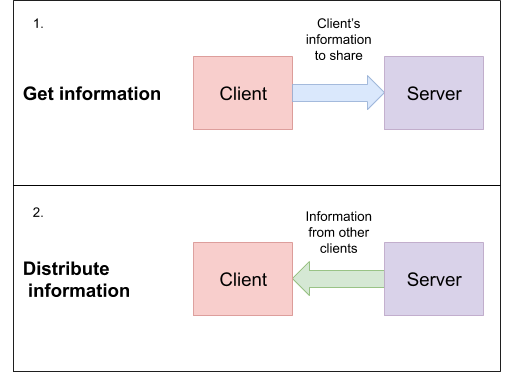
\includegraphics[width=0.6\linewidth]{07_iifo/images/Information_share_graph.png}
    \caption{IIFO and intended contribution information sharing}
    \label{fig:IIFO:information_share_infra}
\end{figure}
\subsection{Disaster Prediction}
\label{subsec:IIFO:disaster_pred}
Each round all agents are asked to share their predictions for when the next disaster happens. Disaster predictions, foraging history and common pool contribution intentions are all discussed in the same format described in \ref{sec:IIFO:implementation}. The information passed allows agents to share information about when they think the next disaster will happen, where it will strike, how strong it will be and how confident they are in their own prediction. The information passed has the format: 
\begin{verbatim}
struct DisasterPredictionInformation = {
   Magnitude = number,
   X,Y = coordinates,
   TimeToPrediction = turns,
   Confidence= percentage
}
\end{verbatim}

\subsection{Foraging History}
\label{subsec:IIFO:foraging_history}
Foraging returns depend on other island's contribution and foraging decisions. It is therefore important to know how much other islands spent on foraging, what resource they foraged and how much they got in return. This information allows agents to update their strategies to take advantage of other client's foraging tactics. The information: below is passed using the pattern described in \ref{sec:IIFO:implementation}
\begin{verbatim}
struct ForagingReturnsInformation = {
   ForagingReturn = resources,
   ForageType = deer or fishing,
   ResourcesSpentOnForaging = resources,
}
\end{verbatim}

